\documentclass[11pt]{article}
\usepackage{fullpage,url}
\usepackage{amsmath,amsthm,amssymb}
\usepackage{graphicx}
\usepackage{eso-pic}
\usepackage{bm}
\usepackage{caption}
\usepackage{picins}   
\usepackage{microtype}
\usepackage{multirow}
\usepackage{url}
\usepackage{enumerate}
%\usepackage{tabular}
\usepackage[letterpaper,top=1in,bottom=1in,left=1in,right=1in,nohead]{geometry}

\newcommand{\PhiB}{\mathbf{\Phi}}
\newcommand{\Ll}{\mathcal{L}}
\newcommand{\Nn}{\mathcal{N}}
\newcommand{\Uu}{\mathcal{U}}
\newcommand{\Ee}{\mathcal{E}}
\newcommand{\Aa}{\mathcal{A}}
\newcommand{\Hh}{\mathcal{H}}
\newcommand{\Ii}{\mathcal{I}}
\newcommand{\Ff}{\mathcal{F}}
\newcommand{\Dd}{\mathcal{D}}
\newcommand{\Tt}{\mathcal{T}}
\newcommand{\Pp}{\mathcal{P}}
\newcommand{\Ss}{\mathcal{S}}
\newcommand{\Cc}{\mathcal{C}}
\newcommand{\Oo}{\mathcal{O}}
\newcommand{\Bb}{\mathcal{B}}
\newcommand{\Rr}{\mathcal{R}}
\newcommand{\Rm}{\mathrm{R}}
\newcommand{\CB}{\mathbf{C}}
\newcommand{\RB}{\mathbf{R}}
\newcommand{\xB}{\mathbf{x}}
\newcommand{\yB}{\mathbf{y}}
\newcommand{\XB}{\mathbf{X}}
\newcommand{\YB}{\mathbf{Y}}
\newcommand{\fB}{\mathbf{f}}
\newcommand{\ZB}{\mathbf{Z}}
\newcommand{\SB}{\mathbf{S}}
\newcommand{\AB}{\mathbf{A}}
\newcommand{\WB}{\mathbf{W}}
\newcommand{\TB}{\mathbf{T}}

\newcommand{\omitme}[1]{}
\newtheorem*{lemma}{Lemma}
\newtheorem{case}{Case}

\makeatletter
\newcommand{\specialnumber}[1]{%
  \def\tagform@##1{\maketag@@@{(\ignorespaces##1\unskip\@@italiccorr#1)}}%
}

\setlength{\parindent}{0in}
\setlength{\parskip}{6pt}

\DeclareMathOperator{\E}{E}
\DeclareMathOperator{\Var}{Var}
\DeclareMathOperator{\Unif}{Unif}

\begin{document}
\thispagestyle{empty}
{\large{\bf CS6957: Probabilistic Modeling \hfill Prateep Mukherjee(u0876583)}}\\

{\LARGE{\bf Homework 3}}
\vspace{0.2\baselineskip}
\hrule

\section{}  
\label{1}

\textbf{\large{NOTE: Please see program p1a.r for part(a) and p1c.r for part(b) and part(c).}}

\begin{figure}[!hbt]
\begin{center}
\[\begin{array}{cc}
 
\includegraphics[scale=0.72]{markov_res.png}  &
  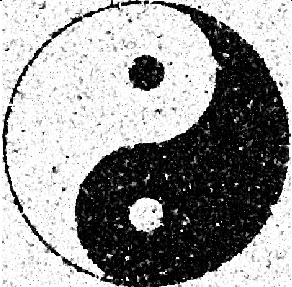
\includegraphics[scale=0.72]{yinyang_res.png} \\
a & b \\
\end{array} \]
\end{center}
\caption{Denoised versions of (a) \textbf{noisy-message.png} and (b) \textbf{noisy-yinyang.png}}
\label{fig1}
\end{figure}

Fig. \ref{fig1} shows the result of Gibbs sampling. For both images, I use 20 \emph{burnin} samples and 100 iterations. For \textbf{noisy-message.png}, I used $\alpha = 0.01$, $\beta = 0.85$, $\sigma = 1.5$. For \textbf{noisy-yinyang.png}, I used $\alpha = 0.01$, $\beta = 1.0$, $\sigma = 1.0$.

%\vspace{-40pt}

\begin{figure}[h]
  \begin{center}
    \[ \begin{array}{cc}
	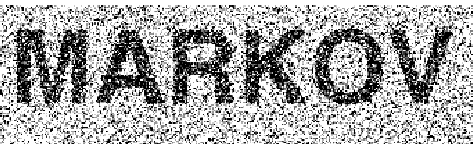
\includegraphics[scale=0.5]{markov_be_0_05.png}  &
	
\includegraphics[scale=0.5]{markov_be_0_5.png} \\
(a) & (b) \\
	
\includegraphics[scale=0.5]{markov_be_0_85.png} &
	
\includegraphics[scale=0.5]{markov_be_2_85.png}  \\
 (c) & (d) \\
    \end{array} \]
  \end{center}
\vspace{-10pt}
\caption{Results obtained by changing values of $\beta$. (a) 0.05, (b) 0.5, (c) 0.85 and (d) 2.85. All other parameters were fixed as mentioned above.}
\label{fig2}
\end{figure}

\par Next, I tested the effects of various values of $\beta$  for \textbf{noisy-message.png}. The results are shown in Fig. \ref{fig2}. The interpretation of $\beta$ is that it penalizes pixels which mismatch. Mismatching pixels form an \textbf{edge} and so we can infer that $\beta$ controls the edges in the cleaned image. Higher values of $\beta$ makes the term $\beta x_i x_j$ term in the energy objective positive, when $x_i \neq x_j$. This penalizes the energy $U$ and makes this step unfavourable. Hence, as we see in Fig \ref{fig2}, increasing $\beta$ values actually loses the edges in the original image. A very low value for $\beta$, on the other hand, hardly removes any noise.(Fig. \ref{fig2}(a)).

\begin{figure}[!hbt]
  \begin{center}
   \[ \begin{array}{ccc}
	 
\includegraphics[scale=0.4]{markov_al_0.png} &
	 
\includegraphics[scale=0.4]{markov_al_0_05.png} &
	 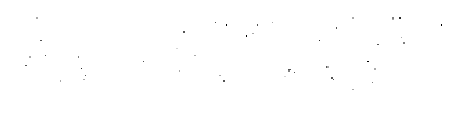
\includegraphics[scale=0.4]{markov_al_2.png} \\
(a) & (b) & (c) \\
     \end{array} \]
  \end{center}
\caption{Results obtained by changing values of $\alpha$ (a) 0, (b) 0.05, (c) 2. All other parameters were fixed as mentioned above.}
\label{fig3}
\end{figure}

\par A similar experiment for $\alpha$ gives us the results shown in Fig. \ref{fig3}. As we increase $\alpha$, more black(=-1) pixels are washed away. 
\vspace{-10pt}
\begin{figure}[!hbt]
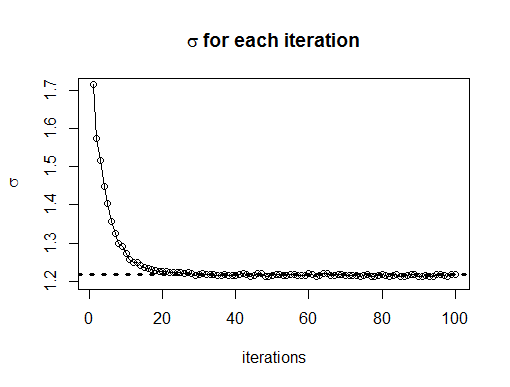
\includegraphics[width=\linewidth]{sigma.png}
\vspace{-20pt}
\caption{$\sigma$ values plotted for each iteration for \textbf{noisy-message.png}. Black dotted line shows convergence value.}
\label{fig4}
\end{figure}
\vspace{-10pt}
\par For question 1(c), I changed the value of $\sigma$ at each iteration using $\sigma_{t} = \sqrt{\frac{|X_{t}-Y|^2}{w \times h}}$, where $X_{t}$ is the image obtained at the $t^{th}$ iteration and $Y$ is the true image. Fig. \ref{fig4} shows the plot of $\sigma$ for the iterations. It converges to a value of $\sim$ 1.2 for \textbf{noisy-message.png} and $\sim$ 1.3 for \textbf{noisy-yinyang.png}.%As expected, the values converge.

\section{}
\label{2}
\textbf{\large{NOTE: Please see program p2.r for this question.}}

\par (a) The formula for un-normalized posterior of $\beta | \YB$ is :

\begin{equation}
   p(\beta| \YB; \XB, \sigma) \propto \prod_{i=1}^{n} [(\frac{1}{1+\exp^{-x_{i}^{T}\beta} })^{y_i} \cdot (\frac{\exp^{-x_{i}^{T}\beta} }{1+\exp^{-x_{i}^{T}\beta} })^{(1-y_i)} ] \cdot \exp{(- \frac{\| \beta \|^2}{2\sigma^2})}
\label{eq1}
\end{equation}

\par (b) Taking logarithm of both sides of Eq. \ref{eq1}, we get 

\begin{eqnarray*}
 log \; \; p( \beta | \YB; \XB, \sigma) &\propto&  \sum_{i=1}^{n} [ -y_i log \; \; (1+\exp^{-x_{i}^{T}\beta} ) \\ 
&+& (1-y_i) log(\exp^{-x_{i}^{T}\beta}) - (1-y_i) log(1+\exp^{-x_{i}^{T}\beta} ) ] - \frac{\| \beta \|^2}{2\sigma^2} \\
&\propto&  - \sum_{i=1}^{n} [(1-y_i) log(\exp^{-x_{i}^{T}\beta}) + log(1+\exp^{-x_{i}^{T}\beta})]+ \frac{\| \beta \|^2}{2\sigma^2}  \\
&\propto& -\sum_{i=1}^{n} (1-y_i)x_{i}^{T}\beta + log(1+\exp^{-x_{i}^{T}\beta}) + \frac{\| \beta \|^2}{2\sigma^2}  \\
&=& U(\beta)
\end{eqnarray*}

Therefore, $p( \beta | \YB; \XB, \sigma) \propto \exp{(-U(\beta))}$.

\par (e) Trace plots for $\beta$ sequence is shown in Fig. \ref{fig5}.

\par (f) The average error rate computed for 40 test samples is on average 0.025.  The values of parameters are $\sigma = 1.0$, $\epsilon = 0.05$, $L = 10$.

\begin{figure}[b]
 \begin{center}
 \[ \begin{array}{cc}
    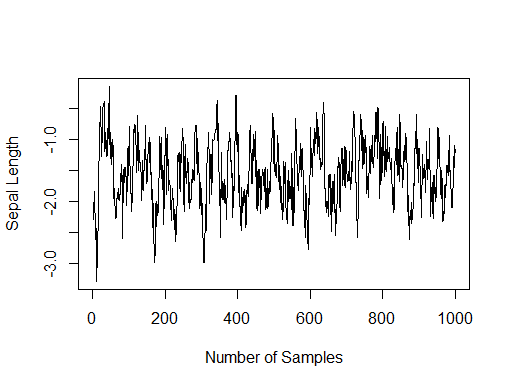
\includegraphics[width=0.5\linewidth]{tr_sl.png} &
    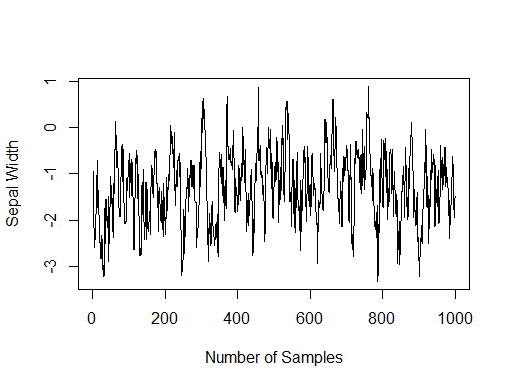
\includegraphics[width=0.5\linewidth]{tr_sw.png} \\
(a) & (b) \\
    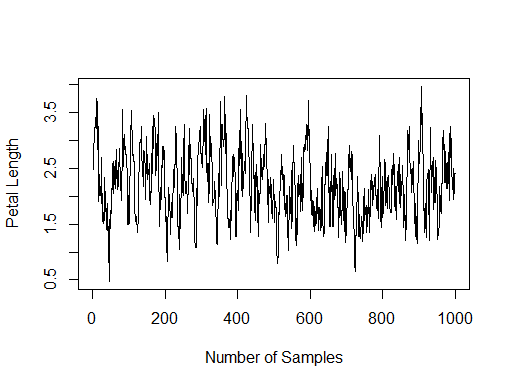
\includegraphics[width=0.5\linewidth]{tr_pl.png} &
    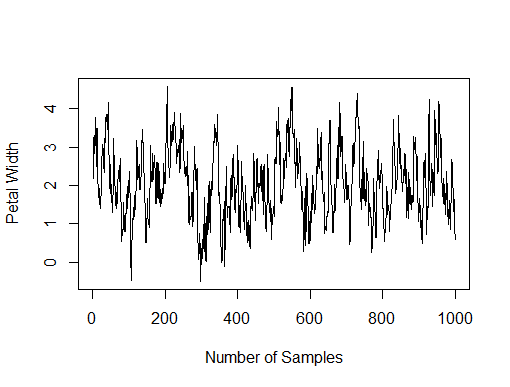
\includegraphics[width=0.5\linewidth]{tr_pw.png} \\
(c) & (d) \\
   \end{array} \]
\vspace{-10pt}
    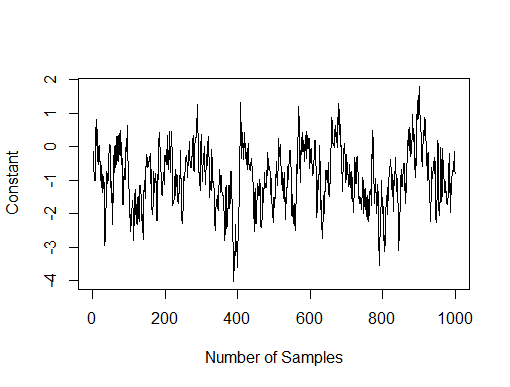
\includegraphics[width=0.5\linewidth]{tr_const.png} \\
(e)
  \end{center}
\vspace{-10pt}
\caption{Trace plots for (a) Sepal length, (b) Sepal width, (c) Petal length, (d) Petal width and (e) Constant term.}
\label{fig5}
\end{figure}  

\end{document}